\chapter{基于点边消息传递网络的复合物筛选模型}
\label{chapter:MPNN}

本章总结了基于结点和基于邻边卷积网络各自的特点,提出了融合特征的重要性。介绍了适合于融合特征的图卷积神经网络算法以及相关消息传递机制的实现。提出了基于点边消息传递网络的复合物筛选模型,并进行了相关的实验与分析。

\section{引言}
\label{section:MPNN:Put}

模型\ref{section:NodeConv:Put}和模型\ref{section:EdgeConv:intro}分别是结点嵌入和邻边嵌入模型,蛋白质复合物的形成和蛋白质特征以及蛋白质互作特征均具有相关性。
无论普通的GCN模型还是EdgeConv模型,均只能直接基于结点特征进行卷积运算,或者邻边特征转换为结点特征之后再进行图卷积运算,这个过程将邻边特征均匀的分配给了其相邻的结点,在模型训练过程邻边作为独立的计算元素依旧缺乏针对邻边本身的更新。这种情形下,邻边特征只能作为结点特征的补充,无法与复合物互作网络动态的结合起来。

为了将邻边特征与结点特征整合到模型的动态参数更新中,本节基于消息传递网络(Message Passing Neural Network,简称MPNN)提出蛋白质复合物特征融合模型,同时处理蛋白质复合物子图中的结点数据和邻边数据,将生物数据、全局拓扑特征以及局部拓扑特征动态的融合起来。
\section{消息传递网络介绍}
\label{section:MPNN:intro}

MPNN网络\cite{gilmer_neural_2017}是一种基于消息传递的图结构学习框架。不同于图卷积模型必须将特征绑定到结点,MPNN将图结构的特征当成消息,特征在结构中的流动被视为消息的传递。在此框架下,图卷积神经网络可以被当作MPNN的特例,是只传递结点消息的MPNN网络。


MPNN网络的具体实现如式\ref{equ:MPNNPassing}所示。

\begin{equation}
    \label{equ:MPNNPassing}
    m_v^{t+1} = \sum_{w \in N_{(v)}}M_t(h_v^t,h_w^t,e_{vw}^t)
\end{equation}
\begin{equation}
    \label{equ:MPNNReadout}
    h_v^{t+1} = U_t(h_v^t,m_v^{t+1})
\end{equation}
其中$N_{(v)}$表示图中结点$v$的邻居,$t$为时间步。公式\ref{equ:MPNNPassing}表示消息传递阶段(Message Passing),$M_t$表示消息传递的更新函数,代表结点w向结点v传递消息的过程中,其传递的消息$h_v^t,h_w^t,e_{vw}$的更新方式。公式\ref{equ:MPNNReadout}表示更新阶段,$U_t$表示更新阶段的函数,代表结点v汇总所有周围消息后的数据更新方式。


\section{基于点边消息传递网络的复合物筛选模型}
\label{section:MPNN:detail}

本节分别介绍基于点边消息传递网络单层更新的具体实现,以及基于该单层更新方法构建的蛋白质复合物评价模型,最后介绍复合物筛选模型的总体实现流程。

\subsection{基于点边消息传递网络单层更新}
\label{section:MPNN:update}
基于点边消息传递网络的复合物筛选模型是基于MPNN网络的改进。
为了使得结点特征和邻边特征具有融合的能力,蛋白质复合物特征融合模型中采用了结点更新邻边,邻边更新结点的方式。在每一层的MPNN过程中,结点t时刻特征更新为邻边t+1时刻特征、邻边t特征更新为结点t+1时刻特征。

结点特征的更新具体方法如下所示。
\begin{equation}
    \label{equ:MineMPNNne}
    ne_v^{t+1} = \frac{\sum_{w \in N_{(v)}}\sigma (Linear^t(e_{vw}^t))}{\left\lVert N_{(v)}\right\rVert }
\end{equation}

\begin{equation}
    \label{equ:MineMPNNnup}
    h_v^{t+1} = Max(h_v^t,ne_v^{t+1})
\end{equation}
式中$Linear$为一层感知器,表示邻边特征的自我更新,$\sigma $为激活函数,本文采用了LeakyRelu函数。式\ref{equ:MineMPNNne}表明了从邻边均值到结点特征的更新过程,$ne_v^{t+1}$为从邻边更新过来的邻边特征,式\ref{equ:MineMPNNnup}表示结点特征结合邻边特征的更新。
可以看出,结点的特征更新来源分为两部分,其一为汇聚所有邻边的特征$e_{vw}^t$,同时为了保留一部分结点中具有关键性的原始特征,其更新方式采用了maxPooling。

邻边特征的具体更新方法如下所示。
\begin{equation}
    \label{equ:MineMPNNen}
    en_{vw}^{t+1} = \sigma (Linear_f^t(m_w^{l} - m_v^{l}) + Linear_s^t m_v^{l})
\end{equation}
\begin{equation}
    \label{equ:MineMPNNeup}
    e_{vw}^{t+1} = Max(e_{vw}^t,en_{vw}^{t+1})
\end{equation}
式中$Linear_f$和$Linear_s$均为感知器,$Linear_f$为对源点到汇点特征流的更新,$Linear_s$为源点特征更新,$en_{vw}^{t+1}$表示依据端点更新的邻边特征。式\ref{equ:MineMPNNeup}表示邻边特征结合结点特征的更新。
从式中得出,类似于结点更新模型,邻边的特征更新也可以分为两部分,分别为邻边自有特征和经过结点特征转换更新的邻边特征,最后同样采用了maxPooling的方式保留关键邻边特征。经过结点特征转换更新的方式综合考虑了源点到汇点的特征流动部分$m_w^{l} - m_v^{l}$以及汇点的特征保留部分$m_v^{l}$。

\subsection{特征子图评价模型}
子图数据保留GO注释特征、拓扑域特征以及亚细胞定位特征等邻边特征,保留Deepwalk特征、GAE特征等结点特征。形成兼具结点和邻边特征的复合物特征子图数据,其中结点特征维度为82维,邻边特征维度维12维。

\begin{figure}[htbp]
    \centering
    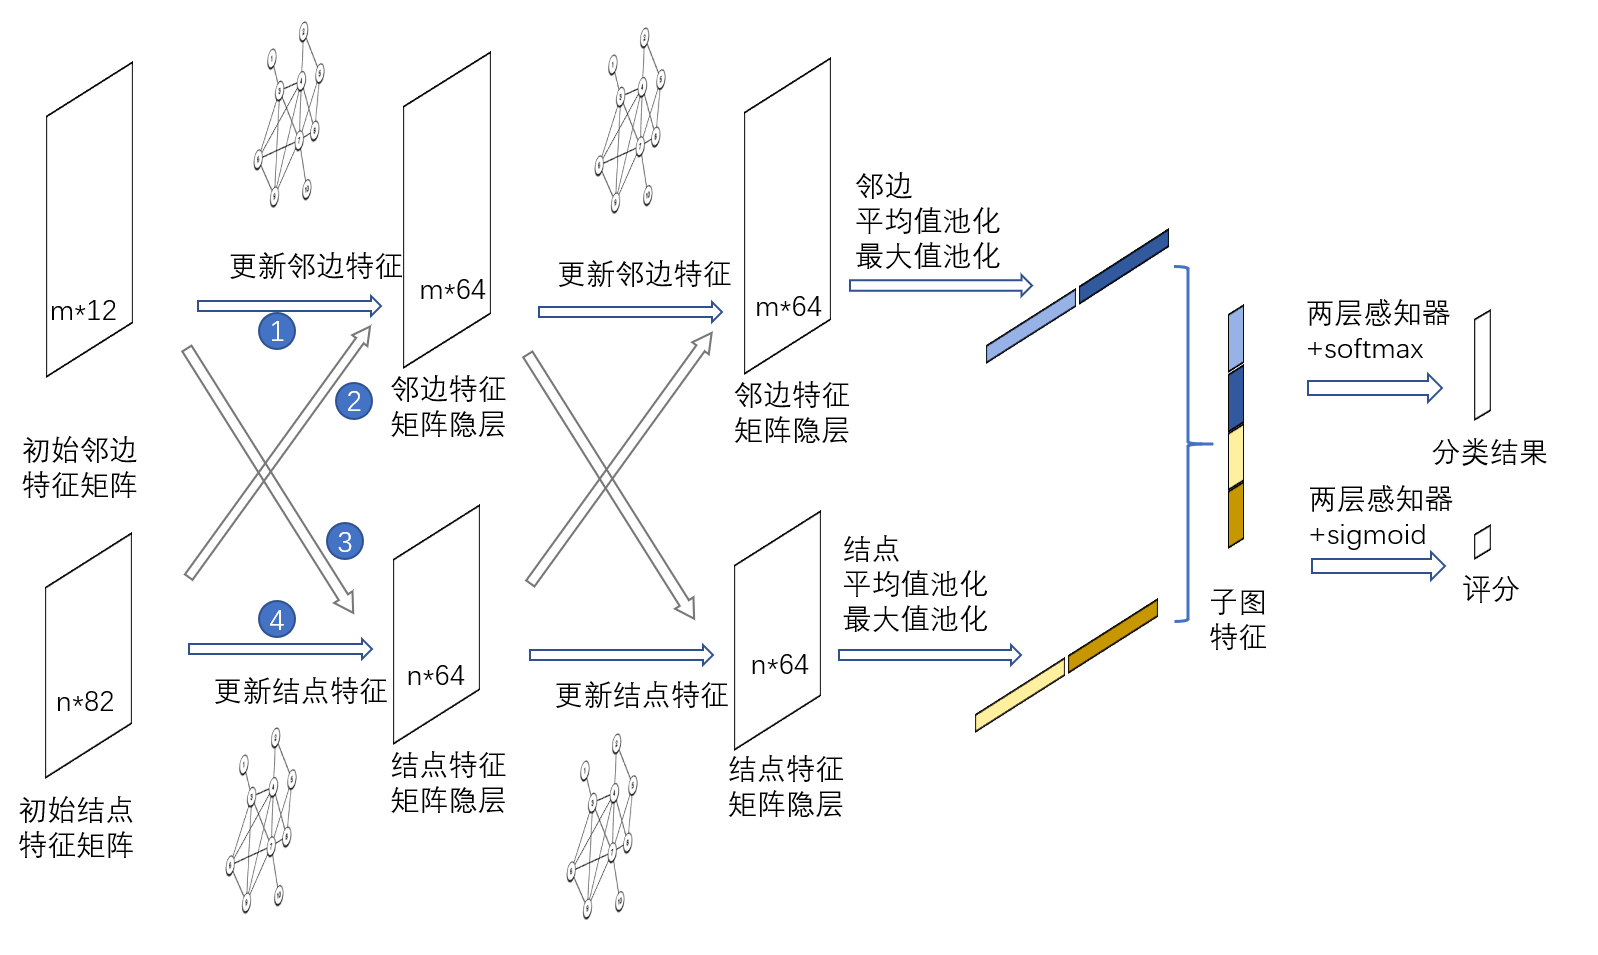
\includegraphics[width=15cm]{mpnn_flow}
    \caption{基于特征融合的分类模型总体流程}
    \label{fig:mpnn_flow}
\end{figure}

在模型中,添加了两层结点和邻边同时更新的MPNN网络,如图\ref{fig:mpnn_flow}所示。每一层MPNN网络中,结点特征更新由结点以及结点周围邻边特征共同确定,如示意图中的结点特征矩阵隐层的数据流所示,过程3是表示通过结点的邻边特征汇聚到一起,再结合过程4结点本身继承上一步的特征,其具体的计算方法如公式\ref{equ:MineMPNNnup}所示。邻边特征更新由邻边以及邻边两侧端点的结点特征共同确定,如示意图中的邻边特征矩阵隐层的数据流所示,过程2表示邻边特征由其源点和汇点特征共同计算,过程1表示邻边特征继承上一步的特征,其具体的计算方法如公式\ref{equ:MineMPNNeup}所示。

消息传递过程中隐层维度设置为64维,两层消息传递之后,采用了对结点特征MaxPooling和MeanPooling的池化方法以及对邻边MaxPooling和MeanPooling的池化方法。一共可以得出四个池化结果,如图中concat到一起之后的四色特征所示,对结果进行拼接之后,形成的256维的特征代表图整体特征。后续分别为两层感知器和softmax层得到图的分类预测,两层感知器和sigmoid层得到图的评分预测。感知器的隐层维度均为64维。

\subsection{筛选模型算法}
本节介绍基于点边消息传递网络的复合物筛选模型的具体算法,包括数据处理,模型训练,样本筛选与结果比对。
具体如算法\ref{alg:mpnngcn-screen}所示。

\begin{algorithm}[h]
    \caption{Protein complex screening model based on MPNN convolution} % 名称
    \label{alg:mpnngcn-screen}
    \begin{algorithmic}[1]
        \Require
        $Com_t$: train protein complexes;
        $Com_b$: protein complexes before screen;
        $Com_g$: golden bench protein complexes;
        $G$: protein-protein interaction network
        \Ensure
        $F1_a,F1_b/SPA_a,SPA_b$: predicted protein complexes F1/SPA metrix after and before screen;
        \State $n$:PIN node number;$m$:PIN edge number;$Com_a=None,layer=2$;
        \State $F_{N} \in \mathbb{R}^{n\times 82}=Concat(F_{GAE},F_{Deepwalk},F_{Self})$;
        \State $F_{E} \in \mathbb{R}^{m\times 14}=Concat(F_{GO},F_{DDI},F_{Subcell},F_{Topo})$;
        \State $Subs_t=Ext(G,F_{N},F_{E},Com_t)$: feated subgraph extract algorithm;
        \For{i=0;i<epoch;i++}
        \For{$BSub_t \in Sub_t$} $loss=0$;
        \For{$Sub_t \in BSub_t$} ~$F_{N}=Linear_in(F_{N}),F_{E}=Linear_ie(F_{E})$;
        \For{$l=0;l<layer;l++$}
        \State $F_{N}^\prime =Mean(Neighbor(\sigma (Linear_m^l(F_{E}))))$;
        \State $F_{E}^\prime =\sigma (Linear_f^l(Flow(F_{N}))+Linear_s^l(Source(F_{N})))$;
        \State $F_{N} =MaxP(F_{N}^\prime,F_{N})$;$F_{E}=MaxP(F_{E}^\prime,F_{E})$;
        \EndFor
        \State $F_t=Concat(MeanP(F_{N}),Maxp(F_{N}),MeanP(F_{E}),Maxp(F_{E}))$;
        \State $PredC_t=MLP_C(F_t)$;$PredS_t=MLP_S(F_t)$;
        \State $loss+=\{CEL(PredC_t,LabelC_t)+\alpha \cdot BCEL(PredS_t,LabelS_t)\}$
        \EndFor; optimization $Adam(loss)$;
        \EndFor
        \EndFor
        \State $Subs_b=Ext(G,F_{N},F_{E},Com_b)$: feated subgraph extract algorithm, see in \ref{section:featSubNetworkConstruct:allSample};
        \For{$Sub_b \in Subs_b$} $PredC_b=MLP_C(F_b)$;$PredS_b=MLP_S(F_b)$;
        \State $Com_a+=Complex(Sub_b)~if~PredC_b=positive|PredS_b>=0.25$;
        \EndFor
        \State $F1_a=F1(Com_a,Com_g),F1_b=F1(Com_b,Com_g)$;
        \State $SPA_a=SPA(Com_a,Com_g),SPA_b=SPA(Com_b,Com_g)$;
    \end{algorithmic}
\end{algorithm}
模型算法中输入数据包括本文\ref{section:featSubNetworkConstruct:allSample}节构造的训练数据集$Com_t$、待筛选数据集$Com_b$以及蛋白质相互作用网络图结构数据,其中训练数据集由蛋白质复合物的正样本数据集,中间样本数据集和负样本数据集构成,训练数据集中每一个蛋白质符合物样本均具有分类标注与评分标注。

模型的输出数据为待筛选数据集筛选之前的所有样本$Com_b$与筛选之后剩余样本$Com_a$的评价指标,评价指标需要参照真实复合物样本集$Com_g$计算,计算的指标包括F1值和综合评价指标SPA。最终的输出为筛选后F1评价指标$F1_a$、筛选前F1评价指标、筛选后SPA评价指标$SPA_a$、筛选前SPA评价指标$SPA_b$,如算法中输出部分所示。

算法中第2行代表基于蛋白质特征嵌入方法的结点特征,其中包括基于图自编码器的16维特征、基于深度随机游走的64维特征和基于蛋白质自有特征嵌入的2维特征,这些特征具体的计算方法如\ref{subsection:featPPINetwork:nodeFeatConstruct}所示,最后经过Concat处理拼接为82维的结点特征矩阵$\mathbb{R}^{n\times 82}$,其中n表示蛋白质相互作用网络中所有结点的数量。第3行代表基于多种蛋白质相似性嵌入方法的邻边特征,其中包括基于GO相似性得到的2维特征$F_{GO}\in \mathbb{R}^{m\times 2}$,基于蛋白质拓扑域相似性得到的7维特征$F_{DDI}\in \mathbb{R}^{m\times 7}$、基于蛋白质亚细胞定位得到的2维特征$F_{Subcell}\in \mathbb{R}^{m\times 2}$和基于拓扑相似性的1维特征,这些特征具体的计算方法如\ref{subsection:featPPINetwork:edgeFeatConstruct}所示,最后经过Concat处理拼接为12维的邻边特征矩阵$\mathbb{R}^{m\times 12}$,其中m表示蛋白质相互作用网络中的所有连边数量。

算法中第4行和第17行表示结合互作网络,特征数据和蛋白质复合物中的蛋白质集合提取取蛋白质复合物特征子图的方法,其中$Subs_t$表示训练数据集提取的所有特征子图,$Subs_b$为待筛选数据集提取的所有特征子图,其具体实现如\ref{section:featSubNetworkConstruct:allSample}所示。

第7行表示特征的初始化,由于结点初始特征和邻边初始特征维度不匹配,为了结点和邻边之间能够进行特征融合,首先需要将其特征统一的转换为64维。
第9行表示基于邻边特征更新结点特征的过程,其中邻边特征进行特征转换与激活,结点特征为其所有邻边特征的均值。
第10行表示基于结点特征更新邻边特征的过程,邻边特征由其两个端点的特征共同确定,分别汇点特征与源点特征形成的数据流以及源点特征自生的更新。
第11行表示特征更新过程中会基于最大值池化保留一部分结点原有特征和邻边原有特征。
算法中第9至11行共同确定了单层的点边消息传递网络更新方式,其具体计算过程如\ref{section:MPNN:update}所示。

算法中第13行表示图读出过程,由于在该模型中邻边特征初始化为了结点特征,同时结点特征经过两层邻边卷积神经网络已经和子图拓扑结构进行了融合,此时结点特征具有较强的表达能力,隐层隐层图读出采用所有结点隐层特征的最大池化$Maxp$和平均池化$Meanp$拼接$Concat$作为子图的特征。

最后第14行表示以基于子图特征的分类预测与评分预测。
第20行至第24行表示基于以训练模型筛选蛋白质复合物样本以及评价阶段。其具体细节如算法\ref{alg:nodegcn-screen}描述所述。

\section{实验设计及结果分析}
\label{section:MPNN:experience}
为了验证基于点边消息传递网络的模型的提升,本文对比了前两章分别设计的基于图卷积神经网络的复合物筛选模型和基于邻边卷积网络的复合物筛选模型。

基于图卷积神经网络的复合物筛选模型是基于研究蛋白质相互作用网络的拓扑结构展开,利用了结点的拓扑特征并基于结点的图卷积神经网络对拓扑特征进行融合,一定程度上体现了$PIN$网络中结点嵌入对复合物预测的作用,证实了复合物中蛋白质在互作网络中相关性对复合物的形成具有一定的影响。

基于邻边卷积网络的复合物筛选模型是基于研究蛋白质之间相似性特征展开,利用了邻边的相似性特征并基于邻边卷积对数据进行融合。生物的相似性数据对复合物预测以及复合物分类具有较明显的提升。

消息传递模型将PIN网络全局特征以及生物特征融合到一起,分别以结点和邻边的形式嵌入到复合物子图中。相较于单独利用其中一方面的模型具有更好的预测能力。为了验证模型的有效性,本章进行了如下的实验。


\subparagraph*{实验方案(一)} 稀疏网络中基于消息传递筛选模型实验

在本文介绍的四个$PPI$网络中,DIP网络的密度最低,为0.0014,其平均度数最低6.98,具有一定的稀疏性。且DIP网络的结点数量较多,为4928个,仅次于Biogrid网络,数据完整性较高。因此方案(一)选择DIP网络作为稀疏网络进行相关实验。

\begin{figure}[htbp]
    \centering
    \subcaptionbox{F1值对比}{\label{fig:dip_f1_fusion}
        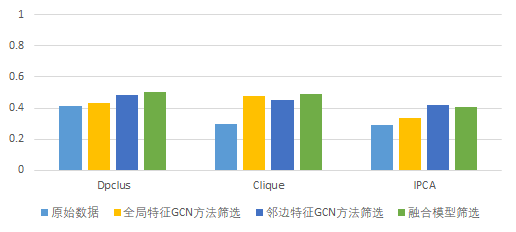
\includegraphics[width=10cm]{dip_f1_fusion}}
    \vskip0.2cm
    \subcaptionbox{SPA值对比}{\label{fig:dip_spa_fusion}
        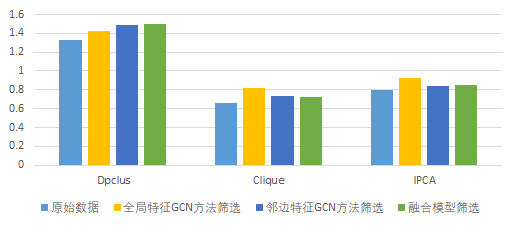
\includegraphics[width=10cm]{dip_spa_fusion}}
    \caption{DIP网络不同模型处理后结果对比}
    \label{fig:dip_fusion}
\end{figure}


\begin{table}[h]
    \centering
    \caption{DIP网络不同模型处理后结果对比数据}
    \begin{tabular}{C{2cm}C{2cm}C{2cm}C{2cm}C{2cm}}
        \toprule
        \textbf{F1值} & \textbf{原始数据} & \textbf{全局特征GCN筛选} & \textbf{邻边特征GCN筛选} & \textbf{融合模型筛选} \\
        \midrule
        Dpclus算法    & 0.414             & 0.434                    & 0.484                    & 0.501                 \\
        Clique算法    & 0.296             & 0.477                    & 0.453                    & 0.487                 \\
        IPCA算法      & 0.291             & 0.336                    & 0.420                    & 0.408                 \\
        \bottomrule
    \end{tabular}
    \begin{tabular}{C{2cm}C{2cm}C{2cm}C{2cm}C{2cm}}
        \toprule
        \textbf{SPA值} & \textbf{原始数据} & \textbf{全局特征GCN筛选} & \textbf{邻边特征GCN筛选} & \textbf{融合模型筛选} \\
        \midrule
        Dpclus算法     & 1.333             & 1.425                    & 1.490                    & 1.498                 \\
        Clique算法     & 0.658             & 0.815                    & 0.731                    & 0.729                 \\
        IPCA算法       & 0.794             & 0.922                    & 0.838                    & 0.848                 \\
        \bottomrule
    \end{tabular}
    \label{tab:result/DIP/fusion}
\end{table}

依据\ref{section:NodeConv:experience}部分中实验方案(一)中提到的方法,针对DIP网络构造了具有四类分类的训练特征子图数据集,基于三种方法生成了待点边消息传递网络的评价模型。模型训练完成之后,分别对三个待筛选特征子图样本数据集中的样本进行了测试并将其中符合要求的复合物保留下来,作为筛选后样本数据集。接下来分别对比了筛选前后样本数据集F1值和综合评价指标。

按照以上的实验方法本章对比了第三章提出的基于图卷积神经网络的复合物筛选模型和第四章提出的基于邻边卷积的蛋白质复合物筛选模型,基于消息传递的模型保留了全局结点特征嵌入和相似性特征嵌入,融合模型具有更精确的蛋白质复合物的评价能力,本章总体的实验结果如下所示。
图\ref{fig:dip_fusion}为在DIP网络中,基于结点的全局特征模型、基于邻边的生物特征模型以及特征融合模型筛选之后结果的对比,包含了F1值对比图和SPA值对比图。表\ref{tab:result/DIP/fusion}为实验结果具体数据。

\subparagraph*{实验方案(二)} 稠密网络中基于消息传递筛选模型实验

在本文介绍的四个$PPI$网络中,Biogrid网络的密度最高,为0.0038,其平均度数最低21.40,远高于其他$PPI$网络,相较于其他网络Biogrid网络稠密性较高。且Biogrid网络的具有最高的结点数量,数据为5573。因此方案(二)选择Biogrid网络作为稠密网络进行相关实验。

\begin{figure}[htbp]
    \centering
    \subcaptionbox{F1值对比}{\label{fig:biogrid_f1_fusion}
        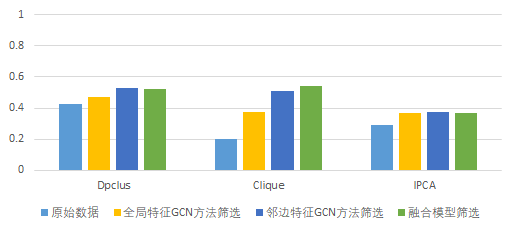
\includegraphics[width=10cm]{biogrid_f1_fusion}}
    \vskip0.2cm
    \subcaptionbox{SPA值对比}{\label{fig:biogrid_spa_fusion}
        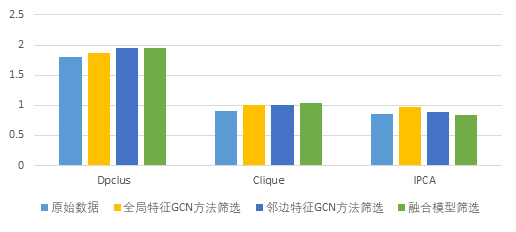
\includegraphics[width=10cm]{biogrid_spa_fusion}}
    \caption{Biogrid网络不同模型处理后结果对比}
    \label{fig:biogrid_fusion}
\end{figure}

\begin{table}[h]
    \centering
    \caption{Biogrid网络不同模型处理后结果对比数据}
    \begin{tabular}{C{2cm}C{2cm}C{2cm}C{2cm}C{2cm}}
        \toprule
        \textbf{F1值} & \textbf{原始数据} & \textbf{全局特征GCN筛选} & \textbf{邻边特征GCN筛选} & \textbf{融合模型筛选} \\
        \midrule
        Dpclus算法    & 0.425             & 0.470                    & 0.529                    & 0.521                 \\
        Clique算法    & 0.203             & 0.373                    & 0.510                    & 0.542                 \\
        IPCA算法      & 0.294             & 0.366                    & 0.373                    & 0.364                 \\
        \bottomrule
    \end{tabular}
    \begin{tabular}{C{2cm}C{2cm}C{2cm}C{2cm}C{2cm}}
        \toprule
        \textbf{SPA值} & \textbf{原始数据} & \textbf{全局特征GCN筛选} & \textbf{邻边特征GCN筛选} & \textbf{融合模型筛选} \\
        \midrule
        Dpclus算法     & 1.796             & 1.871                    & 1.950                    & 1.948                 \\
        Clique算法     & 0.901             & 1.009                    & 1.011                    & 1.041                 \\
        IPCA算法       & 0.859             & 0.970                    & 0.891                    & 0.834                 \\
        \bottomrule
    \end{tabular}
    \label{tab:result/Biogrid/fusion}
\end{table}

依据\ref{section:NodeConv:experience}部分中实验方案(二)中提到的方法,针对Bigrid网络构造了具有四类分类的训练特征子图数据集,基于三种方法生成了待筛选复合物数据集。实验中训练了基于邻边卷积网络的评价模型,并分别对三个待筛选特征子图样本数据集中的样本进行了测试,获取了筛选后样本数据集,最后对比了筛选前后样本数据集F1值和综合评价指标。本章对比了基于图卷积神经网络的复合物筛选模型和基于邻边卷积的蛋白质复合物筛选模型,本章总体的实验结果如下所示。

图\ref{fig:biogrid_fusion}为在Biogrid网络中,基于结点的全局特征模型、基于邻边的生物特征模型以及特征融合模型筛选之后结果的对比,包含了F1值对比图和SPA值对比图。表\ref{tab:result/Biogrid/fusion}为实验结果具体数据。

\subparagraph*{实验结论} ~

从实验方案(一)从图\ref{fig:dip_fusion}中可以看出,在DIP网络中,MPNN融合模型的F1指标在Dpclus和Clique的数据样本中均得到了最优结果,SPA指标在Clique和IPCA算法中有一定降低,而Dpclus算法中SPA指标达到了最优。
和实验方案(二)从图\ref{fig:biogrid_fusion}中可以看出,在Clique样本集上,其SPA指标和F1值均达到了最优结果,在Dpclus的样本集中SPA指标也得到了最优结果。

基于结点和邻边特征融合的复合物筛选模型,对比基于结点特征的图卷积模型和基于邻边特征的邻边卷积模型,其模型更为复杂,筛选的结果中准确率更高。模型在Dpclus和Clique算法中均取得了一定的评价指标效果提升,结果表明了融合特征模型的有效性。


\section{本章小结}
\label{section:MPNN:summary}

本章基于特征融合出发,探讨了融合$PIN$全局特征以及生物相似性特征的情况下,模型设计以及进行了相关的实验。
在特征子图具有GAE和Deepwalk特征等结点特征、多种蛋白质相似性嵌入邻居特征的情况下,本章提出了改进的MPNN更新方法。提出了结点与邻边交替融合更新的模型,详细的阐述了特征子图中交替更新的计算过程以及整体的模型算法。最后本章对比了利用结点特征的基于图卷积的模型,利用相似性特征的基于邻边卷积的模型,实验结果表明融合方法对于数据集中的结果具有一定的提升效果。